\documentclass[conference]{IEEEtran}

\usepackage{cite}
\usepackage{graphicx}

% correct bad hyphenation here
\hyphenation{op-tical net-works semi-conduc-tor}


\begin{document}

\title{Information Centric Networking}

\author{
	\IEEEauthorblockN{
		Andr\'{e} Diegues - 201206858\\
		F\'{a}bio Teixeira - 201305725
	}

	\IEEEauthorblockA{
		T\'{o}picos Avan\c{c}ados em Redes - CC4037\\
		Departamento de Ciencia de Computadores\\
		Faculdade de Ciencias da Universidade do Porto
	}
}

\maketitle

\begin{abstract}
Hoje em dia, o enorme aumento de tr\'{a}fego de conte\'{u}do e dados entre utilizadores na \textit{Internet} motivou o desenvolvimento de novas ideias de arquitetura de \textit{Internet} que resolvam eficazmente este problema. Uma delas \'{e} a que vamos abordar neste artigo, a \textit{Information Centric Networking} (ICN), que atrav\'{e}s de uma abordagem de pesquisa de informa\c{c}\~{a}o nas redes permite fornecer \`{a} rede um servi\c{c}o mais resiliente a falhas que cumpre as exig\^{e}ncias atuais de distribui\c{c}\~{a}o de conte\'{u}do~\cite{ahlgren}. Vamos abordar o seu funcionamento, as arquiteturas que nasceram desta ideia e estudar se a mudan\c{c}a de arquitetura de \textit{Internet} \'{e} ou n\~{a}o vi\'{a}vel. 
\end{abstract}

\section{Introdu\c{c}\~{a}o}
O paradigma ICN foi baseado numa primeira abordagem de arquitetura \textit{Internet} denominada de TRIAD\cite{triad}, cujo principal objectivo seria facilitar e aliviar cerca de 80\% do tr\'{a}fego de \textit{Internet} que servia apenas para entrega de conte\'{u}do atrav\'{e}s de uma arquitetura \textit{data-centric}, isto \'{e}, um utilizador pede o conte\'{u}do ao servidor em vez de pedir ao \textit{host} que det\'{e}m esse mesmo conte\'{u}do\cite{ahlgren}. A TRIAD define uma nova camada de conte\'{u}do que est\'{a} implementada por \textit{content routers} que encaminham os pedidos aos \textit{content servers} que, de seguida, fornecem o conte\'{u}do~.\\

O ICN procura substituir a arquitetura atual, que \'{e} um modelo de comunica\c{c}\~{a}o \textit{host-to-host}, por uma arquitetura baseada num modelo \textit{data-centric}, tratando o conte\'{u}do como entidade principal na arquitetura das redes como podemos observar na figura \ref{icn}. Uma rede com este tipo de arquitetura ganha in\'{u}meras vantagens em rela\c{c}\~{a}o ao modelo \textit{host-to-host}, nomeadamente, na distribui\c{c}\~{a}o de conte\'{u}do, seguran\c{c}a e desenvolvimento de aplica\c{c}\~{o}es\cite{icn}.\\

\begin{figure}[!t]
\centering
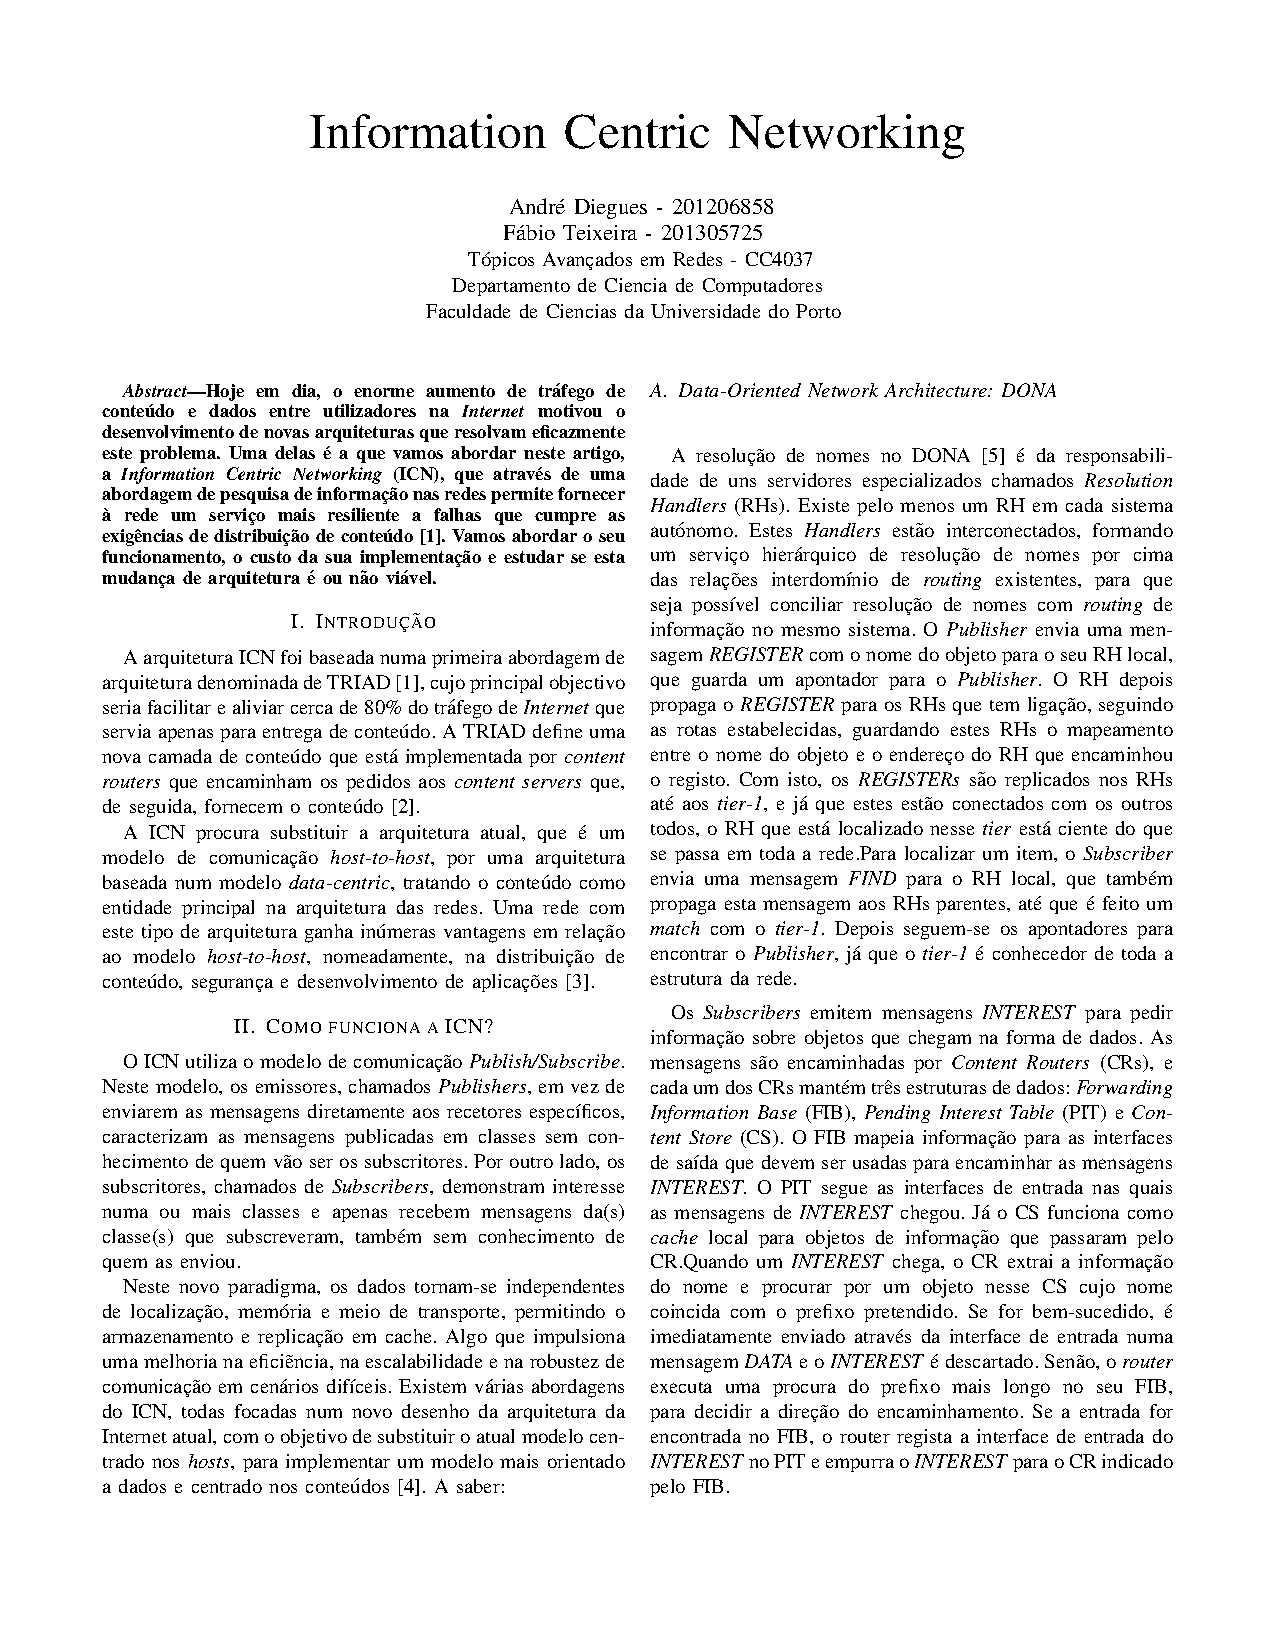
\includegraphics[width=2.5in]{icn}
\caption{Modelo de comunica\c{c}\~{a}o ICN. Retirado de \cite{ahlgren}}
\label{icn}
\end{figure}

Existem v\'{a}rias arquiteturas baseadas neste paradigma. Neste artigo vamos abordar algumas destas arquiteturas, nomeadamente as que ganharam mais apoio ao longo do tempo: \\

\begin{itemize}
\item \textit{Data-Object Network Architecture} (DONA)
\item \textit{Publish-Subscribe Internet Technology} (PURSUIT)
\item \textit{Named Data Networking} (NDN) baseada em \textit{Content-Centric Networking} (CCN) 
\end{itemize}



\section{Como funciona o ICN?}

O ICN utiliza o modelo de comunica\c{c}\~{a}o \textit{Publish/Subscribe}. Neste modelo, os emissores, chamados \textit{Publishers}, em vez de enviarem as mensagens diretamente aos recetores espec\'{i}ficos, caracterizam as mensagens publicadas em classes sem conhecimento de quem v\~{a}o ser os subscritores. Por outro lado, os subscritores, chamados de \textit{Subscribers}, demonstram interesse numa ou mais classes e apenas recebem mensagens da(s) classe(s) que subscreveram, tamb\'{e}m sem conhecimento de quem as enviou.\\ 

Neste novo paradigma, os dados tornam-se independentes de localiza\c{c}\~{a}o, mem\'{o}ria e meio de transporte, permitindo o armazenamento e replica\c{c}\~{a}o em \textit{cache}. Algo que impulsiona uma melhoria na efici\~{e}ncia, na escalabilidade e na robustez de comunica\c{c}\~{a}o em cen\'{a}rios dif\'{i}ceis. Existem v\'{a}rias abordagens do ICN, todas focadas num novo desenho da arquitetura da Internet atual, com o objetivo de substituir o atual modelo centrado nos \textit{hosts}, para implementar um modelo mais orientado a dados e centrado nos conte\'{u}dos\cite{surveyICN}. A saber:\\



\subsection{DONA}

A resolu\c{c}\~{a}o de nomes no DONA\cite{dona} \'{e} da responsabilidade de uns servidores especializados chamados \textit{Resolution Handlers} (RHs). Existe pelo menos um RH em cada sistema aut\'{o}nomo. Estes \textit{Handlers} est\~{a}o interconectados, formando um servi\c{c}o hier\'{a}rquico de resolu\c{c}\~{a}o de nomes por cima das rela\c{c}\~{o}es interdom\'{i}nio de \textit{routing} existentes, para que seja poss\'{i}vel conciliar resolu\c{c}\~{a}o de nomes com \textit{routing} de informa\c{c}\~{a}o no mesmo sistema. O \textit{Publisher} envia uma mensagem \textit{REGISTER} com o nome do objeto para o seu RH local, que guarda um apontador para o \textit{Publisher}. O RH depois propaga o \textit{REGISTER} para os RHs que tem liga\c{c}\~{a}o, seguindo as rotas estabelecidas, guardando estes RHs o mapeamento entre o nome do objeto e o endere\c{c}o do RH que encaminhou o registo.\\

 Com isto, os \textit{REGISTERs} s\~{a}o replicados nos RHs at\'{e} aos~\textit{tier-1}, e j\'{a} que estes est\~{a}o conectados com os outros todos, o RH que est\'{a} localizado nesse \textit{tier} est\'{a} ciente do que se passa em toda a rede.Para localizar um item, o \textit{Subscriber} envia uma mensagem \textit{FIND} para o RH local, que tamb\'{e}m propaga esta mensagem aos RHs parentes, at\'{e} que \'{e} feito um \textit{match} com o~\textit{tier-1}. Depois seguem-se os apontadores para encontrar o \textit{Publisher}, j\'{a} que o \textit{tier-1} \'{e} conhecedor de toda a estrutura da rede. A figura \ref{dona} ilustra como funciona esta arquitetura.\\


%'''CCN (Content Centric Networking project. [Online]. Available: http://www.ccnx.org/)'''[[Image:|top]]



\begin{figure}[!t]
\centering
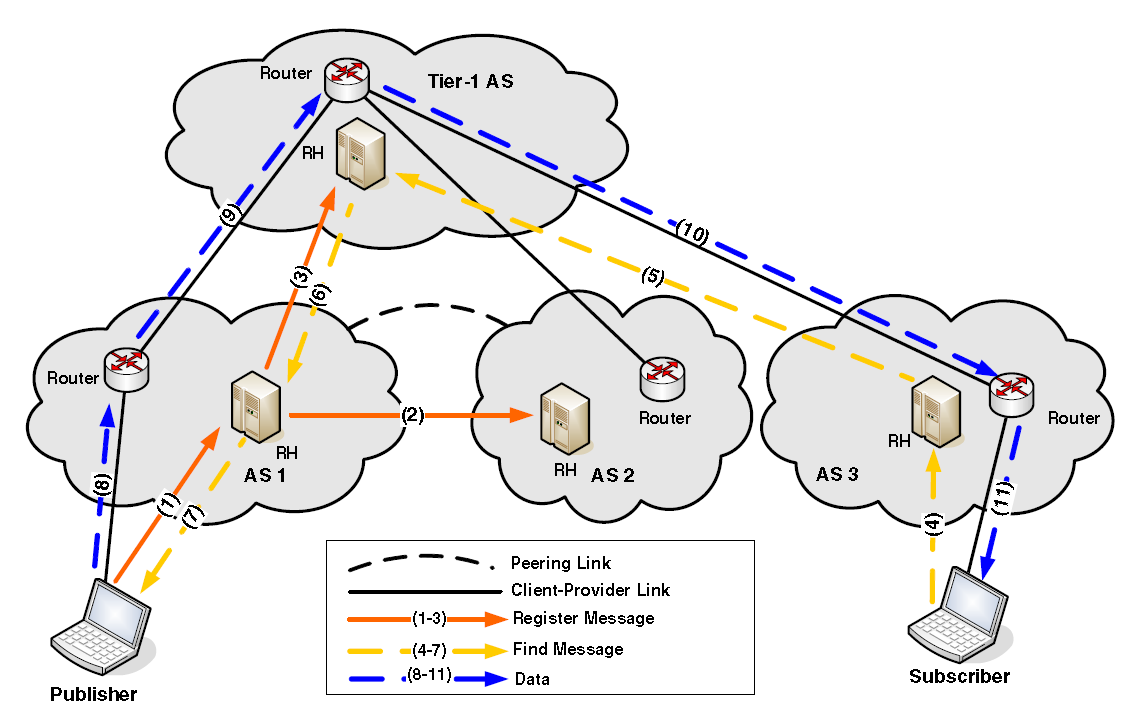
\includegraphics[width=2.5in]{dona}
\caption{Arquitetura DONA. Retirado de \cite{surveyICN}}
\label{dona}
\end{figure}

%'''PURSUIT (FP7 PURSUIT project. [Online]. Available: http://www.fp7-pursuit.eu/PursuitWeb/)'''[[Image:|top]]
\subsection{PURSUIT}

Esta arquitetura substitui completamente a \textit{stack} do protocolo IP por uma \textit{stack} do protocolo \textit{publish-subscribe}. Consiste em tr\^{e}s fun\c{c}\~{o}es distintas: \textit{rendezvous}, \textit{topology management} e \textit{forwarding}.
Quando o \textit{rendezvous} encontra a subscri\c{c}\~{a}o de uma publica\c{c}\~{a}o, direciona a fun\c{c}\~{a}o de gest\~{a}o da topologia para criar uma rota entre o \textit{Publisher} e o \textit{Subscriber}. Esta rota \'{e} usada pela fun\c{c}\~{a}o de encaminhamento para realizar a transfer\^{e}ncia de dados.\\

A resolu\c{c}\~{a}o de nomes no \textit{PURSUIT} \'{e} tratada pela fun\c{c}\~{a}o \textit{rendezvous}, a qual \'{e} implementada por uma cole\c{c}\~{a}o de \textit{Rendezvous Nodes} (RNs), pertencentes \`{a} \textit{Rendezvous Network} (RENE). Quando um \textit{Publisher} quer anunciar um objeto de informa\c{c}\~{a}o, emite uma mensagem \textit{PUBLISH} para o RN local, o qual \'{e} encaminhado por tabelas de \textit{hash} distribu\'{i}das para o RN atribu\'{i}do com o ID do \textit{scope} correspondente. Quando o \textit{Subscriber} emite um \textit{SUBSCRIBE} para o mesmo objeto de informa\c{c}\~{a}o ao seu RN local, \'{e} encaminhado pela tabela de \textit{hash} para o mesmo RN. Depois, o RN informa um n\'{o} da \textit{Topology Management} (TM) para criar uma rota ligando o \textit{Publisher} ao \textit{Subscriber} para entrega de dados. A gest\~{a}o da topologia envia a rota ao \textit{Publisher} numa mensagem \textit{START PUBLISH}, que j\'{a} utiliza a rota para enviar o objeto de informa\c{c}\~{a}o via \textit{Forwarding Nodes} (FNs), vejamos o examplo da figura \ref{pursuit}.\\

\begin{figure}[!t]
\centering
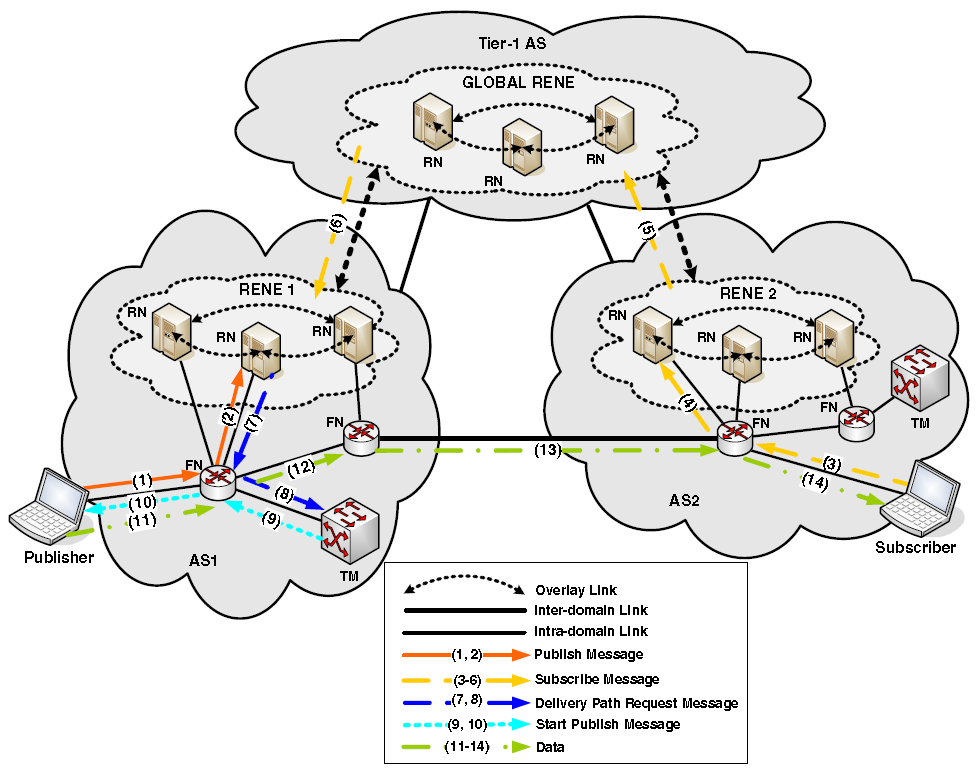
\includegraphics[width=2.5in]{pursuit}
\caption{Arquitetura PURSUIT. Retirado de \cite{surveyICN}}
\label{pursuit}
\end{figure}


\subsection{NDN}

Os \textit{Subscribers} emitem mensagens \textit{INTEREST} para pedir informa\c{c}\~{a}o sobre objetos que chegam na forma de dados. As mensagens s\~{a}o encaminhadas por \textit{Content Routers} (CRs), e cada um dos CRs mant\'{e}m tr\^{e}s estruturas de dados: \textit{Forwarding Information Base} (FIB), \textit{Pending Interest Table} (PIT) e \textit{Content Store} (CS). \\

O FIB mapeia informa\c{c}\~{a}o para as interfaces de sa\'{i}da que devem ser usadas para encaminhar as mensagens \textit{INTEREST}. O PIT segue as interfaces de entrada nas quais as mensagens de \textit{INTEREST} chegou. J\'{a} o CS funciona como \textit{cache} local para objetos de informa\c{c}\~{a}o que passaram pelo CR.Quando um \textit{INTEREST} chega, o CR extrai a informa\c{c}\~{a}o do nome e procurar por um objeto nesse CS cujo nome coincida com o prefixo pretendido. Se for bem-sucedido, \'{e} imediatamente enviado atrav\'{e}s da interface de entrada numa mensagem \textit{DATA} e o \textit{INTEREST} \'{e} descartado. Sen\~{a}o, o \textit{router} executa uma procura do prefixo mais longo no seu FIB, para decidir a dire\c{c}\~{a}o do encaminhamento. Se a entrada for encontrada no FIB, o router regista a interface de entrada do \textit{INTEREST} no PIT e empurra o \textit{INTEREST} para o CR indicado pelo FIB. O exemplo da figura \ref{ndn} permite observar como \'{e} feita a transmiss\~{a}o de conte\'{u}do.\\

\begin{figure}[!t]
\centering
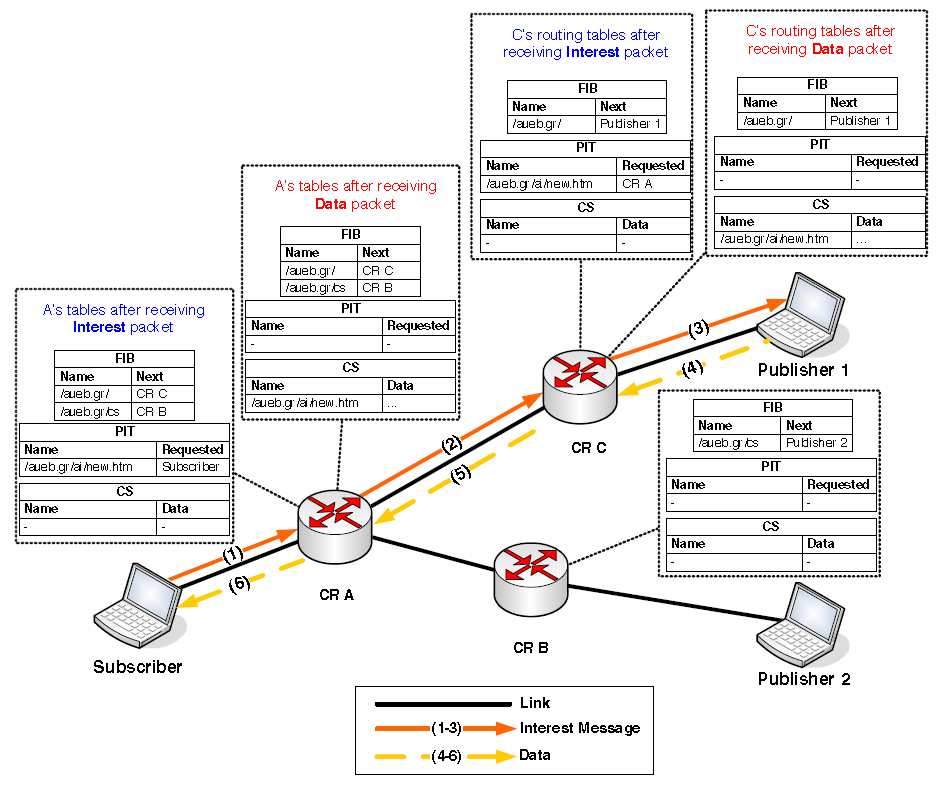
\includegraphics[width=2.5in]{ndn}
\caption{Arquitetura NDN. Retirado de \cite{surveyICN}}
\label{ndn}
\end{figure}

\subsection{Tr\'{a}fego da \textit{Internet} e m\'{e}tricas usadas no ICN}

Analisar o tr\'{a}fego da \textit{Internet} \'{e} importante para perceber que modelo de funcionamento deve ser adotado. Vamos abordar o Labovitz10 
%([https://tools.ietf.org/html/rfc7945#ref-Labovitz10 https://tools.ietf.org/html/rfc7945#ref-Labovitz10])
, um estudo realizado a larga escala, com o prop\'{o}sito de estudar o tr\'{a}fego dos \textit{links} na rede da \textit{Internet}. O resultado indica um dom\'{i}nio claro do tr\'{a}fego \textit{Web}, correspondente a mais de 30\% do tr\'{a}fego total. No entanto, t\'{e}cnicas de \textit{Deep Packet Inspection} (DPI) revelam que entre 13 a 21 porcento do tr\'{a}fego atrav\'{e}s do protocolo HTTP se deve a tr\'{a}fego de v\'{i}deos. J\'{a} a percentagem de tr\'{a}fego \textit{Peer-to-Peer} (P2P) situa-se entre os 17\% e os 19\%.
%<div style="text-align:center;">[[Image:|top]]</div><div style="text-align:center;"><span style="color:#000000;">Percentagem de cada tipo de tr\'{a}fego na Internet</span></div><span style="color:#000000;">
A IETF 
%(</span><span style="color:#000000;">''Internet Engineering Task Force''</span><span style="color:#000000;">)
 tem trabalhado h\'{a} mais de uma d\'{e}cada em desenvolver m\'{e}tricas e m\'{e}todos para medir a \textit{performance} das redes IP. O trabalho foi realizado em grande parte dentro das m\'{e}tricas do IPPM
 %(</span><span style="color:#000000;">''IP Performance Metrics''</span><span style="color:#000000;">) -</span> [https://tools.ietf.org/html/rfc2330 https://tools.ietf.org/html/rfc2330]<span style="color:#000000;">
. As m\'{e}tricas do IPPM incluem atrasos, a varia\c{c}\~{a}o dos mesmos, perdas, reordena\c{c}\~{o}es e duplica\c{c}\~{a}o. Enquanto o trabalho do IPPM for baseado em redes IP ''packet-switched'', isto \'{e}, um m\'{e}todo de comunica\c{c}\~{a}o de rede digital que agrupa todos os dados transmitidos em blocos de tamanho adequado, chamados de pacotes, que s\~{a}o transmitidos atrav\'{e}s de um meio que pode ser compartilhado por v\'{a}rias sess\~{o}es de comunica\c{c}\~{a}o simultâneas
%(</span>[https://en.wikipedia.org/wiki/Packet_switching https://en.wikipedia.org/wiki/Packet_switching]<span style="color:#000000;">)
, \'{e} conceb\'{i}vel que possa ser modificado e estendido para tamb\'{e}m cobrir as redes do ICN. No entanto s\~{a}o necess\'{a}rios mais estudos para transformar essa afirma\c{c}\~{a}o em certeza. Muitos especialistas t\^{e}m trabalhado na reinventa\c{c}\~{a}o e refina\c{c}\~{a}o das m\'{e}tricas e m\'{e}todos IPPM, algo que pode ser ben\'{e}fico para medir o desempenho do ICN. Como estas m\'{e}tricas j\'{a} trabalham em redes ''host-centric'', em compara\c{c}\~{a}o com o ICN implicaria apenas adicionar a extens\~{a}o do mesmo ao quadro IPPM. Um benef\'{i}cio importante de medir o desempenho de transporte de uma rede no seu ''output'', usando m\'{e}tricas baseadas na qualidade de servi\c{c}o (QoS), \'{e} que tal pode ser conseguido, em grande parte, sem qualquer depend\^{e}ncia de aplica\c{c}\~{o}es. Outra op\c{c}\~{a}o para medir a performance de transporte seria usar m\'{e}tricas baseadas em QoS, n\~{a}o ao n\'{i}vel do ''output''<, mas sim ao n\'{i}vel o 'input'' da aplica\c{c}\~{a}o. Para um ''streaming'' de um v\'{i}deo ao vivo, as m\'{e}tricas utilizadas seriam a lat\^{e}ncia de in\'{i}cio, o atraso de ''playout'' e a efici\^{e}ncia na continuidade. Os benef\'{i}cios desta abordagem \'{e} a abstra\c{c}\~{a}o dos detalhes do transporte de rede, o que pode ser ben\'{e}fico quando comparado com diferentes conceitos e tipos de rede. A desvantagem desta abordagem \'{e} a sua depend\^{e}ncia em rela\c{c}\~{a}o \`{a}s aplica\c{c}\~{o}es, sendo por isso prov\'{a}vel que os diferentes tipos de aplica\c{c}\~{o}es exijam diferentes m\'{e}tricas. Pode ser poss\'{i}vel identificar m\'{e}tricas-padr\~{a}o para cada tipo de aplica\c{c}\~{a}o, por\'{e}m \'{e} mais claro utilizar m\'{e}tricas IPPM.

\section{Quais os obst\'{a}culos e custos de implementa\c{c}\~{a}o o ICN?}



\subsection{\textit{Vantagens vs Custo de Implementa\c{c}\~{a}o}}

Nesta sec\c{c}\~{a}o vamos abordar se as vantagens que o ICN traz s\~{a}o fortes o suficiente para motivar uma mudan\c{c}a de arquitetura na \textit{Internet}.\\

Como sabemos, o tr\'{a}fego para entrega de conte\'{u}do tem vindo a aumentar significativamente ao longo dos \'{u}ltimos 5 a 10 anos, de tal modo que foram desenvolvidas solu\c{c}\~{o}es, a curto prazo, para lidar com esta quest\~{a}o, nomeadamente, as \textit{Content Distribution Networks} (CDNs)\cite{cdn} e o \textit{Peer-to-Peer Networking} (P2P)\cite{p2p}, que representam um novo modelo de comunica\c{c}\~{a}o baseado no conte\'{u}do que \'{e} transportado.\\

Assim sendo, haver\'{a} a necessidade de alterar toda a arquitetura da \textit{Internet} por uma arquitetura baseada em ICN? A resposta n\~{a}o \'{e} imediatamente sim, por\'{e}m n\~{a}o s\'{o} o crescimento de tr\'{a}fego \'{e} um dado que vai pesar bastante na resposta, pois significa que a atual arquitetura n\~{a}o representa corretamente a sua utiliza\c{c}\~{a}o, como as CDNs e o P2P n\~{a}o s\~{a}o solu\c{c}\~{o}es perfeitas ao problema, o que poder\'{a} levar a que se considere de forma mais s\'{e}ria a abordagem ICN.\\ 


\begin{figure}[h]
\centering
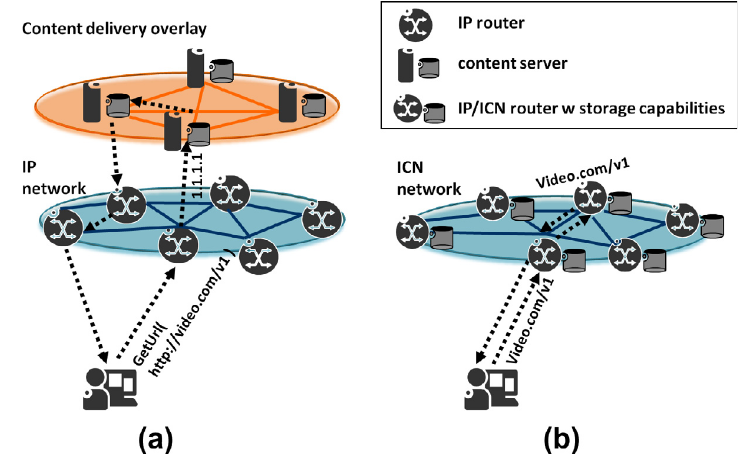
\includegraphics[width=2.5in]{cdnvsicn}
\caption{(a) CDN vs (b) ICN. Retirado de \cite{cdnToICN}}
\label{cdnvsicn}
\end{figure}

O que podemos ganhar com uma arquitetura baseada em ICN\cite{ahlgren}:\\

\begin{enumerate}
\item \textbf{Distribui\c{c}\~{a}o de conte\'{u}do eficiente e escal\'{a}vel} \\

Segundo \cite{icnForest}, esta vantagem por si s\'{o} n\~{a}o \'{e} suficiente para motivar a mudan\c{c}a de arquitetura mas, como j\'{a} referimos acima, se a quantidade de tr\'{a}fego e replica\c{c}\~{a}o de conte\'{u}do continuar a aumentar o ICN \'{e} a melhor estrat\'{e}gia a adotar. \\

\item \textbf{\textit{Naming} \'{u}nico e persistente}\\

Os \textit{Uniform Resource Identifications} (URIs) s\~{a}o localizadores de objetos que exibem o endere\c{c}o IP de um servidor \textit{web} que responde a pedidos resolvendo a parte local de um URI, logo, se um objeto for movido o seu \textit{site} muda de dom\'{i}nio ou o \textit{site} fica \textit{unreachable} quebrando o \textit{naming} do objeto.\\
Outro problema \'{e} se existirem c\'{o}pias do mesmo objeto em diferentes servidores \textit{web} essas c\'{o}pias v\~{a}o ter diferentes URIs, o que \'{e} um desperd\'{i}cio visto que se trata do mesmo objeto.\\

Com o ICN, isto j\'{a} n\~{a}o acontece pois \'{e} poss\'{i}vel atribuir um nome \'{u}nico e persistente aos NDOs e com o modelo de servi\c{c}o que separa produtores de consumidores.
\\

\item \textbf{Modelo de Seguran\c{c}a}\\

A seguran\c{c}a nas redes, hoje em dia, protege a comunica\c{c}\~{a}o entre dois utilizadores, na maior parte das vezes entre cliente e servidor, usando protocolos criptogr\'{a}ficos. Este modelo exige que o cliente confie a entrega da sua informa\c{c}\~{a}o ao servidor.\\

O modelo de seguran\c{c}a do ICN fornece integridade de nome-dados e verifica\c{c}\~{a}o da origem dos NDOs. Garante tamb\'{e}m integridade e autenticidade atrav\'{e}s \textit{caching} ub\'{i}quo.\\ 

\item \textbf{Mobilidade e \textit{Multihoming}}\\

As redes, como as conhecemos hoje em dia, t\^{e}m problemas de gest\~{a}o das liga\c{c}\~{o}es \textit{end-to-end} e na escolha da rota destas liga\c{c}\~{o}es.\\

O ICN n\~{a}o tem estes problemas pois n\~{a}o necessita desta gest\~{a}o de liga\c{c}\~{o}es. O que acontece \'{e} que o cliente continua a fazer \textit{requests} de um novo acesso que possivelmente \'{e} servido por outro servidor em vez de ter de manter uma liga\c{c}\~{a}o do servidor anterior. Da mesma forma, um cliente \textit{multi-homed} pode escolher enviar \textit{requests} a um ou mais acessos.\\

\item \textbf{Toler\^{a}ncia a ruturas}\\

Comunica\c{c}\~{a}o \textit{end-to-end} com transporte de sess\~{o}es para servidores de origem \'{e} muito dificultada em redes de conetividade esparsa, mobilidade veloz e com ruturas.\\

Se o principal objectivo \'{e} aceder a conte\'{u}do, o ICN oferece armazenamento com \textit{in-network caching} para transporte \textit{hop-by-hop}. Este mecanismo d\'{a} garantias de \textit{performance} e fiabilidade.\\

\end{enumerate} 

Migrar da atual estrutura da \textit{Internet} para o ICN s\'{o} ser\'{a} poss\'{i}vel utilizando uma topologia de rede realista. Estas podem ser inferidas atrav\'{e}s de rastreios de \textit{Internet}, como a CAIDA Macroscopic Internet Topology Data Kit 
%([http://www.caida.org/data/active/internet-topology-data-kit])
ou a Rocketfuel.\\
% ([http://www.cs.washington.edu/research/networking/rocketfuel])
 

No entanto, existem problemas associados como o tamanho da topologia (aproximadamente 45 mil sistemas aut\'{o}nomos e perto de 200 mil \textit{links}), o que pode limitar a escalabilidade da ferramenta de avalia\c{c}\~{a}o. Tal como nas topologias \textit{host-centric}, definir apenas um grafo de n\'{o}s n\~{a}o vai ser suficiente. É preciso tamb\'{e}m definir e listar as respetivas matrizes a que correspondem a rede e a \textit{storage} e as capacidades computacionais dispon\'{i}veis para cada n\'{o}, tal como as caracter\'{i}sticas (e atrasos) de cada \textit{link}%([https://tools.ietf.org/html/rfc7945#ref-Montage https://tools.ietf.org/html/rfc7945#ref-Montage])
. Valores aproximados podem ser estimados a partir de plataformas como o iPlane. %([http://iplane.cs.washington.edu/ http://iplane.cs.washington.edu]<span style="color:#000000;">).</span>\\
\\

\subsection{Desafios}

O ICN ainda est\'{a} longe de estar pronto a ser implementado. Os \textit{researchers} t\^{e}m lidado com v\'{a}rios desafios para tornarem este novo modelo dispon\'{i}vel para poder ser colocado ao servi\c{c}o dos utilizadores. Entre os desafios que t\^{e}m encontrado destacam-se\cite{challenges}:\\

\begin{enumerate}


\item \textbf{\textit{Naming} dos dados}\\

Dar nomes aos dados \'{e} t\~{a}o importante para o ICN como dar nomes aos \textit{hosts} \'{e} para a Internet de hoje. Sendo assim, o ICN requer nomes \'{u}nicos para os \textit{Named Data Objects} (NDOs), j\'{a} que os nomes s\~{a}o utilizados para identificar objetos independentemente da sua localiza\c{c}\~{a}o ou conte\'{u}do. Usar tabelas de \textit{hash} \'{e} uma forma poss\'{i}vel de resolver este imbr\'{o}glio, j\'{a} que permite depois que se possa comparar isso com o pr\'{o}prio nome do componente.\\

\item \textbf{Prote\c{c}\~{a}o da privacidade}\\

Como a rede pode ver quem faz o pedido pela informa\c{c}\~{a}o e j\'{a} que a tend\^{e}ncia do ICN \'{e} guardar a hist\'{o}ria dos utilizadores, torna-se um problema para o utilizador n\~{a}o ter garantias de privacidade, j\'{a} que como os nomes devem ter um longo tempo de uso, seria uma limita\c{c}\~{a}o desperdi\c{c}ar nomes.\\

\item \textbf{Atualiza\c{c}\~{o}es}\\

Se um NDO pode ser replicado e guardado na rede para futuros tratamentos, os nomes t\^{e}m de ter um prazo de validade longa e o conte\'{u}do do nome n\~{a}o deve ser alterado, o que impossibilita a atualiza\c{c}\~{a}o de objetos.\\

\item \textbf{Integridade dos dados}\\

A verifica\c{c}\~{a}o da integridade dos dados \'{e} um passo importante para a consolida\c{c}\~{a}o do ICN. O facto de os NDOs n\~{a}o s\'{o} serem recuperados a partir da copa original como tamb\'{e}m a partir de qualquer ponto da rede em que estejam guardados em cache e de poderem ser modificados faz com que n\~{a}o se possa confiar a 100\% na integridade dos dados. Utilizar uma \textit{hash} como parte do nome de objeto \'{e} tamb\'{e}m uma poss\'{i}vel solu\c{c}\~{a}o deste problema, embora a utiliza\c{c}\~{a}o de chaves criptogr\'{a}ficas seja melhor aplicada nestes casos.\\

\item \textbf{\textit{Encryption}}\\

\'{E} poss\'{i}vel cifrar NDOs no ICN e apenas os consumidores que tiverem as chaves podem aceder a esse conte\'{u}do privado. No entanto distribuir e gerir estas chaves, tal como fornecer as interfaces para os utilizadores \'{e} ainda uma mat\'{e}ria de estudo.\\

\item \textbf{Agrega\c{c}\~{a}o e filtragem de tr\'{a}fego}\\

Uma mensagem de um pedido \textit{request} para receber um objeto de dados pode agregar v\'{a}rios pedidos de v\'{a}rios consumidores. Esta agrega\c{c}\~{a}o reduz o tr\'{a}fego na rede, mas torna a filtragem mais dif\'{i}cil. O desafio neste caso \'{e} fornecer um mecanismo que pretenda agrega\c{c}\~{a}o, mas ao mesmo tempo uma pr\'{e}-filtragem dos \textit{request} dos utilizadores. Uma poss\'{i}vel solu\c{c}\~{a}o \'{e} indicar o conjunto de utilizadores que fizeram o \textit{request} nesse \textit{request} agregado, permitindo assim gerar numa resposta apenas o subconjunto dos utilizadores que fizeram \textit{request} e t\^{e}m acesso aos dados. No entanto, esta solu\c{c}\~{a}o requer a utiliza\c{c}\~{a}o de outros n\'{o}s na rede e n\~{a}o permite fazer \textit{caching}.\\

\item \textbf{Roteamento pelo nome}\\

Uma vez que o n\'{u}mero de objetos de dados tem tend\^{e}ncia a aumentar, o tamanho das tabelas de encaminhamento \'{e} um problema a pensar, pois pode ser proporcional ao n\'{u}mero de objetos de dados, a menos que seja introduzido um mecanismo de agrega\c{c}\~{a}o. Por outro lado, o \textit{Route-By-Name Routing} (RBNR) reduz a lat\^{e}ncia e simplifica o processo de roteamento devido \`{a} omiss\~{a}o do processo de resolu\c{c}\~{a}o.\\
\end{enumerate}


\subsection{Testes de trabalhos anteriores}

Na sec\c{c}\~{a}o anterior vimos que o \textit{caching} poderia manter os dados continuamente dispon\'{i}veis na rede. Alguns \textit{researchers} investigaram o assunto realizando testes de \textit{performance} sobre as v\'{a}rias formas de fazer \textit{caching}.

% teste de centrality caching e porque e que ubiquity caching e pior Cache “Less for More” in Information-Centric Networks 

% tipos de caching Caching in information centric networking: A survey

% Probabilistic In-Network Caching for Information-Centric Networks ∗

% Age-based Cooperative Caching in Information-Centric Networking

% bandwidth testes Modeling in-network caching and bandwidth sharing performance in information-centric networking & Bandwidth and Storage Sharing Performance in Information Centric Networking

% Hash-routing Schemes for Information Centric Networking - hashing

% Information centric networking over SDN and OpenFlow: Architectural aspects and experiments on the OFELIA testbed

% Economic Incentives in Information- Centric Networking: Implications for Protocol Design and Public Policy
\section{ICN: O futuro da \textit{Internet}}

Os utilizadores est\~{a}o cada vez mais interessados em receber conte\'{u}dos, seja qual for a sua origem, do que ter de aceder a um servidor para receber essa informa\c{c}\~{a}o. E o facto de a \textit{Internet} ainda ser centrada nos \textit{hosts} implica que o utilizador tenha de especificar em cada pedido n\~{a}o s\'{o} a informa\c{c}\~{a}o que deseja receber, como tamb\'{e}m especificar o servidor do qual a informa\c{c}\~{a}o pode ser retirada. Com o ICN isso j\'{a} n\~{a}o acontece\cite{surveyICN}.\\

O pressuposto b\'{a}sico por tr\'{a}s do ICN \'{e} que a informa\c{c}\~{a}o \'{e} nomeada, endere\c{c}ada e encontra o conte\'{u}do independentemente da sua localiza\c{c}\~{a}o. Uma implica\c{c}\~{a}o indireta da implementa\c{c}\~{a}o do ICN \'{e} que a informa\c{c}\~{a}o se torna orientada para o recetor, em contraste com a atual realidade da Internet em que os emissores t\^{e}m controlo total sobre os dados trocados\cite{publishSubscribe}. No ICN s\'{o} s\~{a}o recebidos os dados que o recetor tenha pedido. Depois de ser enviado o pedido, a rede \'{e} respons\'{a}vel por localizar a melhor origem para fornecer a informa\c{c}\~{a}o desejada ao recetor.\\

Quando um elemento da rede receber um pedido por conte\'{u}do, pode ter duas a\c{c}\~{o}es: se estiver em \textit{cache}, responde imediatamente com o conte\'{u}do; se n\~{a}o estiver, faz um pedido aos elementos com os quais tem liga\c{c}\~{a}o e depois guardar em \textit{cache} o conte\'{u}do quando for encontrado\cite{surveyICN}.\\

Nesse sentido, e j\'{a} que os conte\'{u}dos chegam de elementos da rede ao inv\'{e}s da origem, o desenho do ICN tem de garantir a seguran\c{c}a dos conte\'{u}dos, contrariamente \`{a} estrutura atual da Internet que se foca no caminho. Para isso, quem fornece os dados assina um modelo de seguran\c{c}a para que os elementos da rede e os consumidores apenas tenham de verificar essa assinatura para garantir a sua fiabilidade\cite{icnForest}.\\


\section{Conclus\~{a}o}
The conclusion goes here.\\
%From content delivery today to information centric networking

\IEEEtriggeratref{8}
\IEEEtriggercmd{\enlargethispage{-5in}}

\bibliography{icn}
\bibliographystyle{IEEEtran}

\end{document}


